\documentclass[a4paper,12pt]{article}

\usepackage[utf8x]{inputenc}
\usepackage[T2A]{fontenc}
\usepackage[english, russian]{babel}

% Опционно, требует  apt-get install scalable-cyrfonts.*
% и удаления одной строчки в cyrtimes.sty
% Сточку не удалять!
% \usepackage{cyrtimes}

% Картнки и tikz
\usepackage{graphicx}
\usepackage{tikz}
\usetikzlibrary{snakes,arrows,shapes}


% Некоторая русификация.
\usepackage{misccorr}
\usepackage{indentfirst}
\renewcommand{\labelitemi}{\normalfont\bfseries{--}}

% Увы, поля придётся уменьшить из-за листингов.
\topmargin -1cm
\oddsidemargin -0.5cm
\evensidemargin -0.5cm
\textwidth 17cm
\textheight 24cm

\sloppy

% Оглавление в PDF
\usepackage[
bookmarks=true,
colorlinks=true, linkcolor=black, anchorcolor=black, citecolor=black, menucolor=black,filecolor=black, urlcolor=black,
unicode=true
]{hyperref}

% Для исходного кода в тексте
\newcommand{\Code}[1]{\texttt{#1}}

\usepackage{verbatim}
\usepackage{fancyvrb}
\fvset{frame=leftline, fontsize=\small, framerule=0.4mm, rulecolor=\color{darkgray}, commandchars=\\\{\}}
\renewcommand{\theFancyVerbLine}{\small\arabic{FancyVerbLine}}


\title{Отчёт по лабораторной работе \\ <<Динамическая IP-маршрутизация>> \\ Вариант №37}
\author{(Кузьмин А.Ю. ИУ7-39)}

\begin{document}

\maketitle

\tableofcontents

\section{Настройка сети}

\subsection{Топология сети}

Топология сети и используемые IP-адреса показаны на рисунке~\ref{fig:network}.

\begin{figure}
\centering
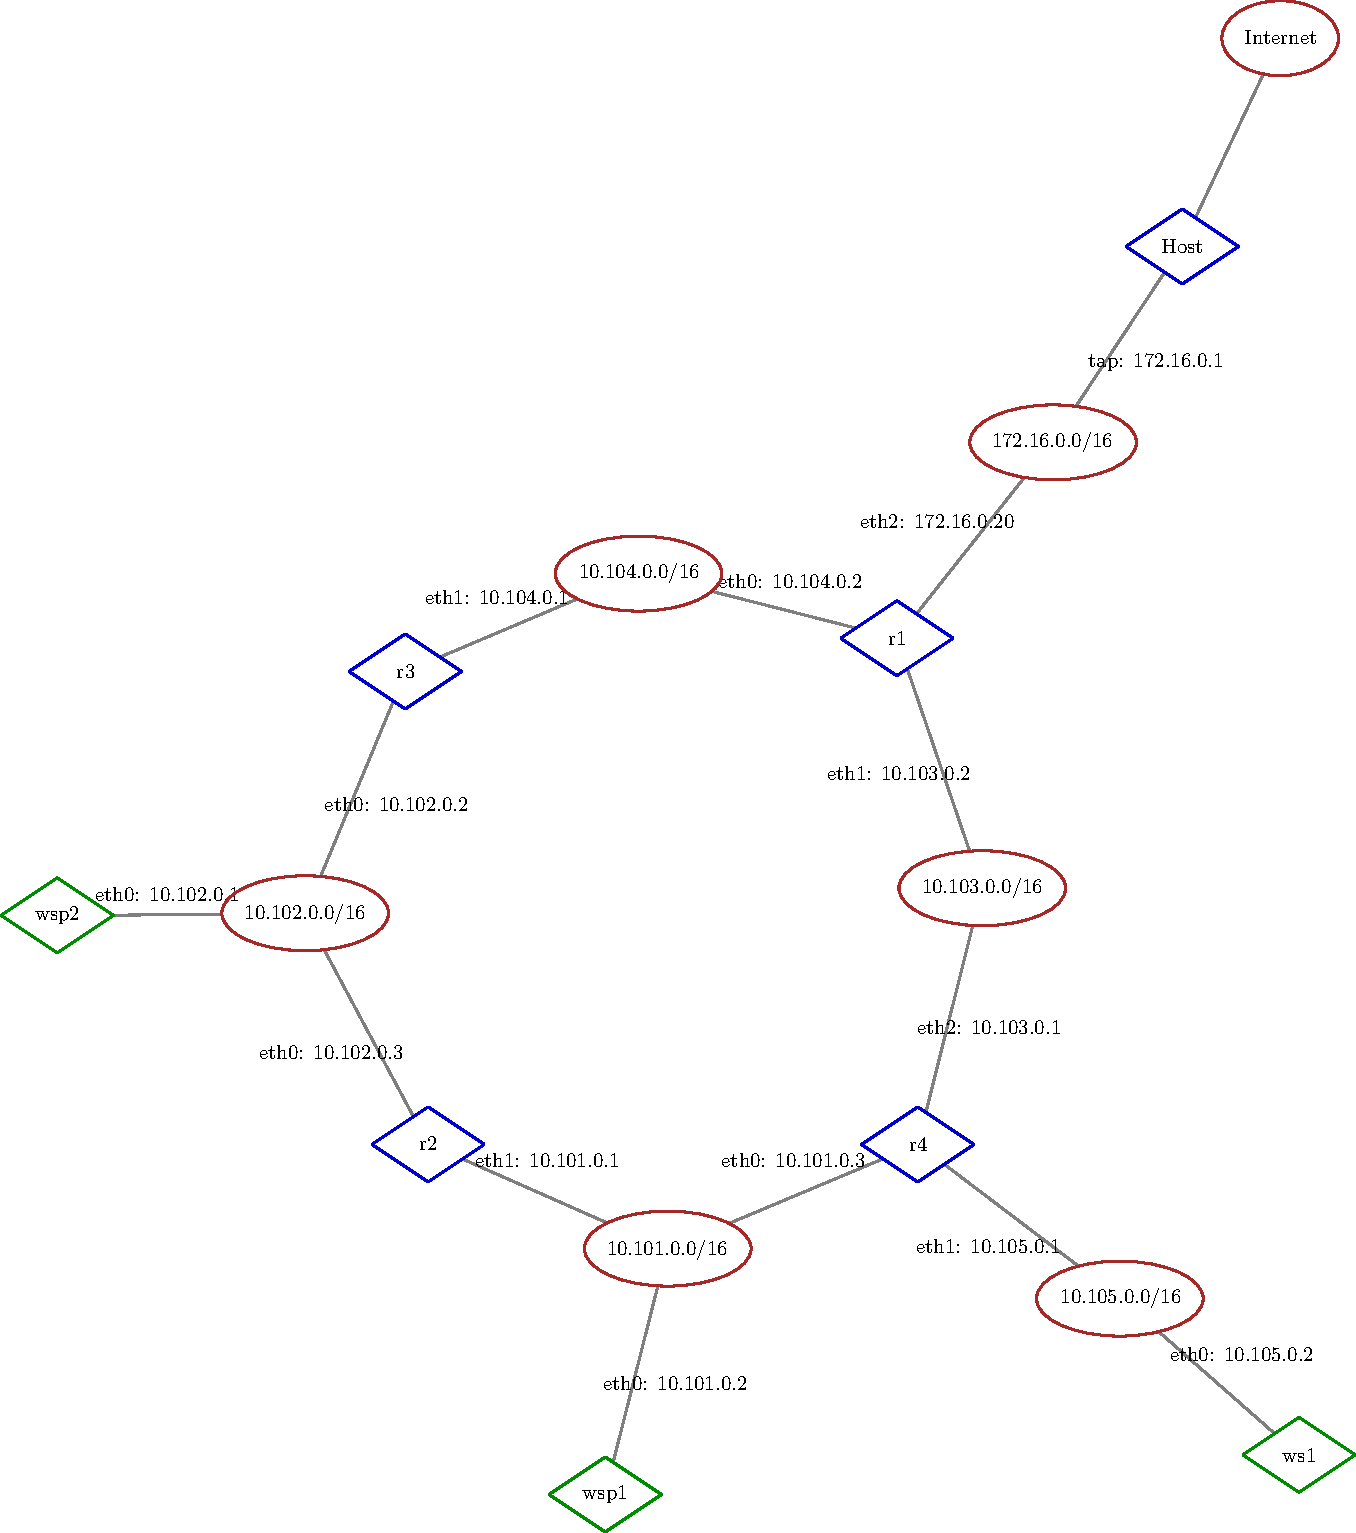
\includegraphics[width=0.8\textwidth]{includes/network_gv.pdf}
\caption{Топология сети}
\label{fig:network}
\end{figure}

Перечень узлов, на которых используется динамическая IP-маршрутизация: r1, r2, r3, r4, wsp1, wsp2


\subsection{Назначение IP-адресов}

Ниже приведён файл сетевой настройки  маршрутизатора r1.

\begin{Verbatim}
auto lo
iface lo inet loopback

auto eth0
iface eth0 inet static
address 10.104.0.2
netmask 255.255.0.0

auto eth1
iface eth1 inet static
address 10.103.0.2
netmask 255.255.0.0
\end{Verbatim}

Ниже приведён файл сетевой настройки  маршрутизатора r2.

\begin{Verbatim}
auto lo
iface lo inet loopback

auto eth0
iface eth0 inet static
address 10.102.0.3
netmask 255.255.0.0

auto eth1
iface eth1 inet static
address 10.101.0.1
netmask 255.255.0.0
\end{Verbatim}

Ниже приведён файл сетевой настройки  маршрутизатора r3.

\begin{Verbatim}
auto lo
iface lo inet loopback

auto eth0
iface eth0 inet static
address 10.102.0.2
netmask 255.255.0.0

auto eth1
iface eth1 inet static
address 10.104.0.1
netmask 255.255.0.0
\end{Verbatim}

Ниже приведён файл сетевой настройки  маршрутизатора r4.

\begin{Verbatim}
auto lo
iface lo inet loopback

auto eth0
iface eth0 inet static
address 10.101.0.3
netmask 255.255.0.0

auto eth1
iface eth1 inet static
address 10.105.0.1
netmask 255.255.0.0

auto eth2
iface eth2 inet static
address 10.103.0.1
netmask 255.255.0.0
\end{Verbatim}

Ниже приведён файл сетевой настройки рабочей станции ws1.

\begin{Verbatim}
auto lo
iface lo inet loopback

auto eth0
iface eth0 inet static
address 10.105.0.2
netmask 255.255.0.0
gateway 10.105.0.1
\end{Verbatim}

Ниже приведён файл сетевой настройки рабочей станции wsp1.

\begin{Verbatim}
auto lo
iface lo inet loopback

auto eth0
iface eth0 inet static
address 10.101.0.2
netmask 255.255.0.0
\end{Verbatim}

Ниже приведён файл сетевой настройки рабочей станции wsp2.

\begin{Verbatim}
auto lo
iface lo inet loopback

auto eth0
iface eth0 inet static
address 10.102.0.1
netmask 255.255.0.0
\end{Verbatim}



\subsection{Настройка протокола RIP}

Ниже приведен файл \Code{/etc/quagga/ripd.conf} маршрутизатора r1.

\begin{Verbatim}
router rip

network eth0
network eth1

timers basic 10 60 120

redistribute kernel
redistribute connected

log file /var/log/quagga/ripd.log
\end{Verbatim}

Ниже приведен файл \Code{/etc/quagga/ripd.conf} маршрутизатора r2.

\begin{Verbatim}
router rip

network eth0
network eth1

timers basic 10 60 120

redistribute kernel
redistribute connected

log file /var/log/quagga/ripd.log
\end{Verbatim}

Ниже приведен файл \Code{/etc/quagga/ripd.conf} маршрутизатора r3.

\begin{Verbatim}
router rip

network eth0
network eth1

timers basic 10 60 120

redistribute kernel
redistribute connected

log file /var/log/quagga/ripd.log
\end{Verbatim}

Ниже приведен файл \Code{/etc/quagga/ripd.conf} маршрутизатора r4.

\begin{Verbatim}
router rip

network eth0
network eth2

timers basic 10 60 120

redistribute kernel
redistribute connected

log file /var/log/quagga/ripd.log
\end{Verbatim}

Ниже приведен файл \Code{/etc/quagga/ripd.conf} рабочий станции, связанной с несколькими маршрутизаторами wsp1.

\begin{Verbatim}
router rip

network eth0

timers basic 10 60 120

redistribute kernel
redistribute connected

log file /var/log/quagga/ripd.log
\end{Verbatim}

Ниже приведен файл \Code{/etc/quagga/ripd.conf} рабочий станции, связанной с несколькими маршрутизаторами wsp2.

\begin{Verbatim}
router rip

network eth0

timers basic 10 60 120

redistribute kernel
redistribute connected

log file /var/log/quagga/ripd.log
\end{Verbatim}

\section{Проверка настройки протокола RIP}

Вывод \textbf{traceroute} от узла ws1 до wsp2 при нормальной работе сети.

\begin{Verbatim}
traceroute 10.102.0.1
traceroute to 10.102.0.1 (10.102.0.1), 64 hops max, 40 byte packets
 1  10.105.0.1 (10.105.0.1)  2 ms  0 ms  0 ms
 2  10.101.0.1 (10.101.0.1)  0 ms  0 ms  0 ms
 3  10.102.0.1 (10.102.0.1)  1 ms  0 ms  0 ms
\end{Verbatim}

Вывод \textbf{traceroute} от ws1 до внешнего IP (195.19.38.2).

\begin{Verbatim}
raceroute 195.19.38.2
traceroute to 195.19.38.2 (195.19.38.2), 64 hops max, 40 byte packets
 1  10.105.0.1 (10.105.0.1)  0 ms  0 ms  0 ms
 2  10.103.0.2 (10.103.0.2)  11 ms  1 ms  0 ms
 3  172.16.0.1 (172.16.0.1)  11 ms  1 ms  0 ms
 4  192.168.0.1 (192.168.0.1)  1 ms  1 ms  1 ms
 5  195.19.38.2 (195.19.38.2)  4 ms  1 ms  1 ms
\end{Verbatim}

Вывод сообщения RIP на r2 (eth1).

\begin{Verbatim}
IP (tos 0x0, ttl 1, id 0, offset 0, flags [DF], proto UDP (17), length 112) 10.101.0.3.520 > 224.0.0.9.520: 
        RIPv2, Response, length: 84, routes: 4
          AFI: IPv4:         0.0.0.0/0 , tag 0x0000, metric: 2, next-hop: self
          AFI: IPv4:      10.103.0.0/16, tag 0x0000, metric: 1, next-hop: self
          AFI: IPv4:      10.104.0.0/16, tag 0x0000, metric: 2, next-hop: self
          AFI: IPv4:      10.105.0.0/16, tag 0x0000, metric: 1, next-hop: self
\end{Verbatim}

Вывод таблицы RIP на r2.

\begin{Verbatim}
     Network            Next Hop         Metric From            Tag Time
R(n) 0.0.0.0/0          10.102.0.2            3 10.102.0.2        0 00:53
C(i) 10.101.0.0/16      0.0.0.0               1 self              0
C(i) 10.102.0.0/16      0.0.0.0               1 self              0
R(n) 10.103.0.0/16      10.101.0.3            2 10.101.0.3        0 00:53
R(n) 10.104.0.0/16      10.102.0.2            2 10.102.0.2        0 00:53
R(n) 10.105.0.0/16      10.101.0.3            2 10.101.0.3        0 00:53
\end{Verbatim}

Вывод таблицы маршрутизации на r2.

\begin{Verbatim}
10.101.0.0/16 dev eth1  proto kernel  scope link  src 10.101.0.1 
10.103.0.0/16 via 10.101.0.3 dev eth1  proto zebra  metric 2 
10.102.0.0/16 dev eth0  proto kernel  scope link  src 10.102.0.3 
10.105.0.0/16 via 10.101.0.3 dev eth1  proto zebra  metric 2 
10.104.0.0/16 via 10.102.0.2 dev eth0  proto zebra  metric 2 
default via 10.102.0.2 dev eth0  proto zebra  metric 3 
\end{Verbatim}

\section{Расщепленный горизонт и испорченные обратные обновления}

1) Маршрутизатор r3 (eth0), на r2 включен расщепленный горизонт

\begin{Verbatim}
IP (tos 0x0, ttl 1, id 0, offset 0, flags [DF], proto UDP (17), length 92) 10.102.0.3.520 > 224.0.0.9.520: 
        RIPv2, Response, length: 64, routes: 3
          AFI: IPv4:      10.101.0.0/16, tag 0x0000, metric: 1, next-hop: self
          AFI: IPv4:      10.103.0.0/16, tag 0x0000, metric: 2, next-hop: self
          AFI: IPv4:      10.105.0.0/16, tag 0x0000, metric: 2, next-hop: self
\end{Verbatim}


Маршрутизатор r3 (eth1), на r1 включен расщ. горизонт и испорченные обратные обновления.

\begin{Verbatim}
IP (tos 0x0, ttl 1, id 0, offset 0, flags [DF], proto UDP (17), length 152) 10.104.0.2.520 > 224.0.0.9.520: 
        RIPv2, Response, length: 124, routes: 6
          AFI: IPv4:         0.0.0.0/0 , tag 0x0000, metric: 1, next-hop: self
          AFI: IPv4:      10.101.0.0/16, tag 0x0000, metric: 2, next-hop: self
          AFI: IPv4:      10.102.0.0/16, tag 0x0000, metric: 16, next-hop: 10.104.0.1
          AFI: IPv4:      10.103.0.0/16, tag 0x0000, metric: 1, next-hop: self
          AFI: IPv4:      10.104.0.0/16, tag 0x0000, metric: 16, next-hop: self
          AFI: IPv4:      10.105.0.0/16, tag 0x0000, metric: 2, next-hop: self
\end{Verbatim}


\section{Имитация устранимой поломки в сети}

Выключили маршрутизатор r2.

Вывод таблицы RIP непосредственно перед истечением таймера устаревания (на маршрутизаторе r3).

\begin{Verbatim}
     Network            Next Hop         Metric From            Tag Time
R(n) 0.0.0.0/0          10.104.0.2            2 10.104.0.2        0 00:56
R(n) 10.101.0.0/16      10.102.0.3            2 10.102.0.3        0 00:04
C(i) 10.102.0.0/16      0.0.0.0               1 self              0
R(n) 10.103.0.0/16      10.104.0.2            2 10.104.0.2        0 00:56
C(i) 10.104.0.0/16      0.0.0.0               1 self              0
R(n) 10.105.0.0/16      10.102.0.3            3 10.102.0.3        0 00:04
\end{Verbatim}

Перестроенная таблица на этом же маршрутизаторе

\begin{Verbatim}
     Network            Next Hop         Metric From            Tag Time
R(n) 0.0.0.0/0          10.104.0.2            2 10.104.0.2        0 00:59
R(n) 10.101.0.0/16      10.104.0.2            3 10.104.0.2        0 00:59
C(i) 10.102.0.0/16      0.0.0.0               1 self              0
R(n) 10.103.0.0/16      10.104.0.2            2 10.104.0.2        0 00:59
C(i) 10.104.0.0/16      0.0.0.0               1 self              0
R(n) 10.105.0.0/16      10.104.0.2            3 10.104.0.2        0 00:59
\end{Verbatim}


Вывод \textbf{traceroute} от wsp2 до wsp1 после того, как служба RIP перестроила таблицы маршрутизации.

\begin{Verbatim}
traceroute 10.101.0.2
traceroute to 10.101.0.2 (10.101.0.2), 64 hops max, 40 byte packets
 1  10.102.0.2 (10.102.0.2)  7 ms  0 ms  0 ms
 2  10.104.0.2 (10.104.0.2)  9 ms  0 ms  0 ms
 3  10.103.0.1 (10.103.0.1)  9 ms  1 ms  1 ms
 4  10.101.0.2 (10.101.0.2)  7 ms  1 ms  1 ms
\end{Verbatim}

\section{Имитация неустранимой поломки в сети}

Выключили маршрутизатор r4.

Таблица протокола RIP на маршрутизаторе r1:

\begin{Verbatim}
     Network            Next Hop         Metric From            Tag Time
K(r) 0.0.0.0/0          172.16.0.1            1 self              0
R(n) 10.101.0.0/16      10.103.0.1           16 10.103.0.1        0 01:53
R(n) 10.102.0.0/16      10.104.0.1            2 10.104.0.1        0 00:52
C(i) 10.103.0.0/16      0.0.0.0               1 self              0
C(i) 10.104.0.0/16      0.0.0.0               1 self              0
R(n) 10.105.0.0/16      10.103.0.1           16 10.103.0.1        0 01:53
\end{Verbatim}

\end{document}
